\documentclass[letter]{article}

\usepackage{MD_estilo}

\nombre{Vicente Vial} % Aqui va el nombre del alumno
\numtarea{11} % Aqui va el número de la tarea

\sigla{IIC2343} % Aqui va la sigla del curso
\curso{Arquitectura de computadores} % Aqui va el nombre del curso
\semestre{2} % Aqui va el semestre del curso
\ano{2018} % Aqui va el año del curso


\begin{document}
	
	\begin{pregunta}{1} % Aqui se coloca el número de la pregunta
	
	a) Dispositivos I/O usados:
	$$ $$
	
	1) Timer del sistema: Mandará IRQ cuando se cumpla plazo límite de algún programa.
	
	2) Real Time Clock: Se usará para obtener hora de inicio de programa.
	
	3) Display(Funciones de video): Se usará como dispositivo de output, se activará luego de ocurrir el fin de algún programa, informará a usuario acerca de que el programa finalizó.
	
	4) Disco: Se usará para almacenar programa,y guardarlo en RAM cuando se vaya a usar.
	$$ $$
	b) Procedimiento completo que realiza el mecanismo a alto nivel:
	$$ $$
	1) Primero programa se carga en RAM, se guarda en una variable(en RAM) asociada al programa la hora de Real Time clock, y se guarda en el timer, la hora de término del programa. Todo esto manejado por el sistema operativo.
	
	2) Luego, programa se desarrolla normalmente.
	
	3) En el momento que se termina el tiempo del programa,el timer mandará un IRQ, al ser atendida esta IRQ, el SO buscará en la RAM el programa que haya excedido el tiempo, para esto tiene que analizar cual es el programa que tiene la hora de inicio que haya excedido el tiempo establecido, para luego dar término al programa ejecutado.
	
	4) Al final de la rutina del S0, activada por  interrupción del timer, el SO realizará cambios en el Display(Funciones de video), para informar al usuario acerca del fin del programa.
	
	$$ $$
	
	c)) Para cada uno de los dispositivos utilizados, indique en detalle cómo sería la interacción con  él (tipo de comunicación, instrucciones, modelo de interacción, función de interrupción), desde que comienza su participación en el proceso. 
	$$ $$
	1) Timer del sistema: Primero, el SO modificará variables almacenadas en la memoria del timer del sistema, ingresando un tiempo próximo para una interrupción en una variable en su memoria(más bien será un arreglo con los próximos tiempos a interruptir), esto se realiza medainte mapped I/0. Luego, el Timer, enviará una IRQ al PIC(en hora de interrupción, guardada en arreglo), el PIC, enviará un aviso al CPU*, y enviará devuelta una señal INTA, para luego mandar el ID del timer del sistema. Luego se comienza con la ISR del timer, que básicamente consistirá en avisar al sistema operativo acerca de que un programa excedió el tiempo, posterior a esto, el S0 tomará el control, buscará el programa, y lo finalizará para luego modificar el Diplay (Funciones de video).
	$$ $$
	2) Real Time Clock: este dispositivo, estará constantemente enviando señales a la CPU, las que serán atendidas de la misma forma anterior por el PIC, y su ISR, consistirá en modificar una variable en la RAM, asociada a la hora actual. 
	$$ $$
	3) Display(Funciones de video): El sistema operativo modificará su estado, luego de que se produzca una interrupción del timer, y posteriormente la interrupción de software de interrupción de video, para esto el SO podrá modificar las variables del display (asociadas a lo que se muestra) mediante puertos, usando la instrucción OUT PORT, reg.
	$$ $$
	4) Disco: Este dispositivo, contendrá los programas guardados, y cuando comience el programa, cargará los datos e instrucciones de estos en la RAM, mediante el DMA.
	
	

	
	
	
	
	
	
	
	
	
	
	\end{pregunta}
	
	\begin{pregunta}{2}

$$ $$
a)No tiene sentido, ya que el objetivo de la caché es buscar la información de manera más rápida aprovechando el trade off de tamaño y rápidez, al tener un tamaño superior, se tendría una rápidez menor a la memoria principal, ya que al tener más tamaño sería mas lento buscar. No cambia si es que es igual al tamaño de la memoria direccionable, ya que igualmente sería mas grande o igual al tamaño de la memoria principal.
$$ $$
También se debe considerar igualmente lo siguiente:
$$ $$
"no tiene sentido si se utiliza un esquema donde la memoria caché se ubique después de la
MMU, ya que todas las peticiones de memoria tendrían como límite el tamaño de la memoria principal (CPU sólo conoce tamaño de la memoria principal, no de la caché). Tampoco tiene sentido sacar la memoria principal y dejar la caché como si fuera ahora la principal. Una cach´e no puede funcionar sin la noción de espacio direccionable virtual o espacio direccionable físico, de la manera en que est´a construida una CPU y la caché dentro de ella (la CPU no sabe que existe la caché, sélo los espacios direccionables).Por otro lado, si la caché se ubica antes de la MMU, entonces una caché mayor a la memoria principal
traería ventajas, ya que podría almacenar el contenido de marcos que se encuentran en el swap-file." (PREGUNTA 2b, Interrogación 3, 2016-2)


$$ $$
b) Proporcion donde hubo hit = 0.95

hit time = $12\L^3 - 81L + 68$

Miss Time = cte

E(T) = $0.95(12L^3 - 81L +68)$ + $0.05(12L^3 - 81L +68 + MISS TIME)$

E(T)`= $0.95(36L^2 - 81)$ + $0.05(36L^2 - 81) = 0$ 

E(T)`= $(36L^2 - 81) = 0$

L = $(3/2)$

Finalmente:

L = 2

$$ $$

c) Si podría existir un problema similar, si es que N-way tuviera una línea por conjunto(1-way), en ese caso al tener dos bloques intentando ingresar al conjunto, pelearían por la misma línea. Si es que hubieran más líneas, podría pasar que dos bloques intenten entrar al mismo conjunto,y se peleen por entrar al conjunto, si el sistema es LIFO, se podría dar que se pelee por la línea (con otras línea no utilizadas en la caché).


$$ $$

d) Se podría almacenar la matriz 1 por fila en memoria, y la matriz 2 por columna en memoria, así la primera matriz al estar almacenada por fila, cuando se multiplique el primer elemento de la fila, se guardará en caché elementos de la fila que posteriormente serán multiplicados, y la matriz 2, al guardarse por columna, cuando se multiplique el primer elemento de la columna, se guardarán en caché elementos de la columna que van a ser multiplicados. Esto es útil, ya que la multiplicación de matriz se hace multiplicando las filas de la matriz1 por las columnas de la matriz2. También para aumentar el hit rate, se podría tener una función de correspondencia full asociative, y una politica de que el menos usado sale(LFU), esto ya que columnas de la matriz se dejan de usar luego de multiplicar las filas de la matriz 1.

$$ $$
\end{pregunta}
	
	\begin{pregunta}{3}
	Primero, al haber muchos procesos en ejecución simultánea, podría pasar que se acaben los marcos posibles para asignar a las páginas. Esto se soluciona mediante swapping, es decir, agregando un bit que indique si el marco esta en memoria ó en disco duro. Si el SO quiere asignar un marco y no quedan marcos disponibles, entonces enviará a disco(swapp out) el valor menos usado ó con tiempo de ingreso mas lejano(dependiendo del criterio que se use,fifo,random,lru,lfu,...) y asignara marco a valor actual en memeoria, luego en caso de que el SO intente buscar un valor y  esté disco duro, podrá acceder al valor, regresandolo a memoria(swapp in), y enviando a disco(swapp out) el valor menos usado ó con tiempo de ingreso mas lejano(dependiendo del criterio que se use,fifo,random,lru,lfu,...). Este mecanismo ya se implementa, y requiere un disco duro que respalde algunos marcos asignados a páginas.
	
	Ya solucionado este problema, pueden haber problemas de cantidad de memoria, ya que al haber muchos procesos simultáneamente, la memoria tendrá que almacenar muchas tablas de páginas, y esto limitará el numero de procesos simúltaneos, y además, sucederá que no se tendrá tanta memoria para guardar muchas tablas de páginas. La solución a esto, podría ser, primero, agregar más memoria, y así poder asignar un espacio más grande de memoria para almacenar las tablas de página,se podría además reorganizar la estructura de los datos en memoria, para que se hiciera más espacio para las tablas de página. La segunda solución, es respaldar las tablas de página con un disco duro externo, así cuando un programa necesite usar la tabla de página, primero se buscará si la tabla existe en memoria, y si no se accederá a buscarla al disco, funcionaría similar al swapping, es decir, cuando ya no queda más espacio para que el SO asigne tablas de página, enviará la tabla de página menos usada ó la que fue última vez usada(dependiendo del criterio que se use,fifo,random,lru,lfu,...) a disco duro(swapp out), y llevará a memoria la tabla de página del proceso actual, luego se seguirá el procedimiento normalmente. Si se quiere usar una tabla del disco duro, se hará un swapp(out)de la tabla de página menos usada ó la que fue última vez usada(dependiendo del criterio que se use,fifo,random,lru,lfu,...), y se hará un swapp in de la tabla de página en disco que se quiere usar.
	
	
	

	
	
	
	


    
	\end{pregunta}
	
	
	
	
	
	
	
	
	
	
	
	
	
	
	\begin{pregunta}{4}
	$$ $$
	a) Desventajas pipeline muy profundo:
	
	Una desventaja es  que se tiene el riesgo en términos de la implementacion de la componente de predicción de saltos,  si está se ubica en una etapa cercana al final, su prediccion errónea implicaría una perdida considerable de ciclos perjudicando la eficiencia de la ejecucion del programa paralelizado. Además el uso de energía del computador podría ser excesivo,provocando,por ejemplo, que el computador se caliente, además la ejecución simultanea de tantos programas se vuelve más compleja.(I3-2018-1(pregunta 1.4)

	$$ $$
	b)	Spectre: se refiere a una falla, que se origina porque muchos computadores tienen una unidad predictora de saltos, luego esta unidad deja cierta evidencia de información privada, que sistemas o personas sin autorización pueden dilucidar.
	
	Meltdown: es una falla que ocasiona, que un sistema o persona no autorizado, puedan cualquier línea de la memoria, incluso, la memoria que esta reservada para el modo supervisor.
	
	No se pueden arreglar, por la principal razón de que el hardware ya está implementado(con la unidad de salto incluido), se podría agregar un sistema de seguridad por software, pero seguirá la grieta del sistema.
	
   
	$$ $$
	
	c) Imagen en página siguiente.

	{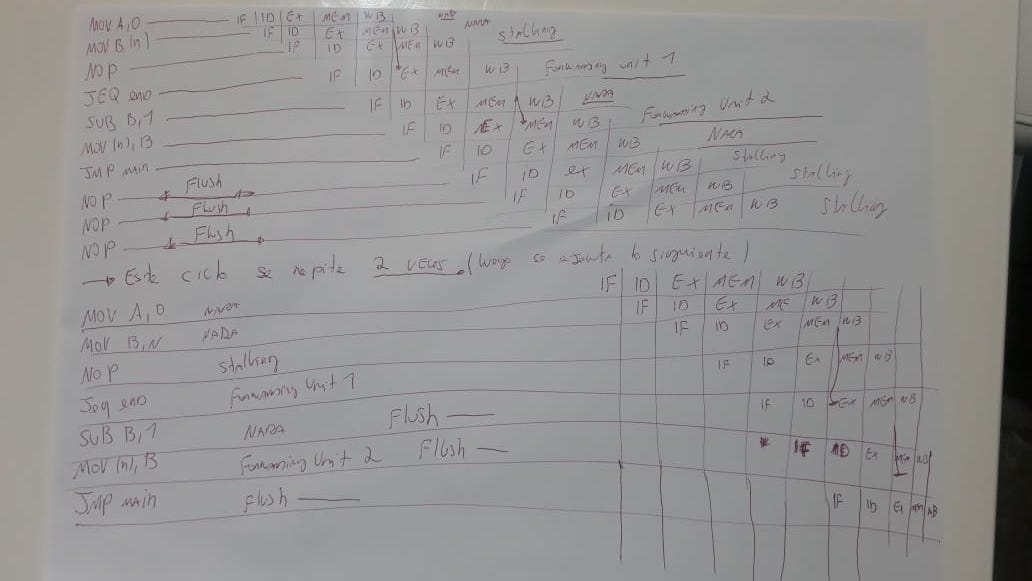
\includegraphics[width=17cm]{p4.jpeg}}
	\end{pregunta}


	\begin{pregunta}{5}
	
	
Cuando un recurso se comparte por primera vez se asigna el estado E para indicar que es exclusivo.
Luego, cuando otro procesador solicita su lectura, se hará la copia del recurso entre cachés, y el estado del recurso de la caché solicitante será de S para ese procesador, y para el primer procesador el estado se convierte en F(para indicar que será el encargado predeterminado para compartir el recurso entre las cachés).Si ninguna de las cachés realiza una modificación, y otra caché solicita el recurso, entonces la caché con el recurso en estado F, compartirá el recurso a cache solicitante, que marcará el registro como S. Posteriormente, si una caché(F ó S) realiza una modificación, la caché que realiza la modificación cambia la línea a estado O y las otras invalidan su copia, pasando a estado I.Luego, si una caché solicita lectura del recurso, la caché que sea dueña del recurso(O), enviará directamente el recurso a las otras caché, que marcarán el recurso como S. 
$$ $$
Si existe sólo una caché con un recurso en estado E, y realiza una modificación sobre el recurso, el recurso cambia a estado M, si otra caché solicita la lectura del recurso, la primera caché enviará recurso a caché solicitante, la primera caché modificará su estado de recurso a O, y la caché solicitante a cambiará su estado a S. (EXAMEN 2018-1(pregunta 5.3), I3-2018-1(pregunta 2.3))



	\end{pregunta}
\end{document}
